この節ではFDPSの概要を記述する。FDPSの開発目的、FDPSの基本的な考えかた、
FDPSを使用して作成したコードの動作について概説する。

%%%%%%%%%%%%%%%%%%%%%%%%%%%%%%%%%%%%%%%%%%%%%%%%%%%%%%%%%%%%%%%%%%%%%%
\subsection{開発目的}

粒子シミュレーションは、重力$N$体シミュレーション、SPHシミュレーション、
渦糸法、MPS法、分子動力学シミュレーションなど理学工学の様々な分野で使
用されている。より大きい空間スケール、より高い空間分解能(または質量分
解能)、より長い時間スケールの物理現象を追跡するために、高性能な粒子シ
ミュレーションコードへの要請はますます強くなっている。

高性能な粒子シミュレーションコードを組むためには、シミュレーションコー
ドの大規模並列化を避けることはできない。粒子シミュレーションコードの大
規模並列化をする際には、ロードバランスのため動的領域分割、領域分割に合
わせた粒子交換、ノード間通信の削減と最適化、キャッシュ利用効率の向上、
SIMDユニット利用効率の向上、アクセラレータへの対応など、数多くの困難な
処理を行う必要がある。現在、研究グループは個別にこれらの処理へ対応して
いる。

しかし、上記の処理は粒子シミュレーション共通のものである。FDPSの開発目
的は、これらの処理を高速に行うライブラリを提供し、大規模並列化への対応
に追われていた研究者の負担を軽くすることである。FDPSを使うことで、研究
者がよりクリエイティブな仕事に専念できるようになれば、幸いである。

%%%%%%%%%%%%%%%%%%%%%%%%%%%%%%%%%%%%%%%%%%%%%%%%%%%%%%%%%%%%%%%%%%%%%%
\subsection{基本的な考えかた}

ここではFDPSの基本的な考えかたについて記述する。

%%%%%%%%%%%%%%%%%%%%%%%%%%%%%%%%%%%%%%%%%%%%%%%%%%%%
\subsubsection{大規模並列粒子シミュレーションの手順}
\label{sec:overview_concept_abstraktion}

まずFDPSにおいて、大規模並列粒子シミュレーションがどのような手順で行わ
れることを想定しているかを記述する。粒子シミュレーションは、以下のよう
な微分方程式を時間発展させるものである。
\begin{align}
    \frac{d\bm{u}_i}{dt} = \sum_j f(\bm{u}_i,\bm{u}_j) + \sum_s
    g(\bm{u}_i,\bm{v}_s) \label{eq:GoverningEquation}
\end{align}
ここで$\bm{u}_i$は粒子$i$の物理量ベクトルであり、この物理量には質量、
位置、速度など粒子が持つあらゆる物理量が含まれる。関数$f$は粒子$j$から
粒子$i$への作用を規定する。以後、作用を受ける粒子を$i$粒子、作用を与え
る粒子を$j$粒子と呼ぶことにする。$\bm{v}_s$は$i$粒子から十分遠方にある
粒子を1つの粒子としてまとめた粒子(以後、この粒子を超粒子と呼ぶ)の物理
量ベクトルである。関数$g$は超粒子から$i$粒子への作用を規定する。式
(\ref{eq:GoverningEquation})の第2項は、重力やクーロン力など無限遠まで
到達する長距離力の場合はゼロではない。しかし流体の圧力のような短距離力
はゼロである。

大規模並列化された粒子シミュレーションコードは以下の手順で式
(\ref{eq:GoverningEquation})を時間発展させる。ここではデータの入出力や
初期化は省略している。
\begin{enumerate}
\item 以下の2段階の手順でどのプロセスがどの粒子の式
  (\ref{eq:GoverningEquation})を時間発展させるか決める。
  \label{item:LoadBalance}
  \begin{enumerate}
  \item プロセスの間でロードバランスを取れるように、シミュレーションで
    扱っている空間の領域を分割し、各プロセスの担当領域を決める(領域分
    割)。
  \item 各プロセスが、自分の担当する領域に存在する全粒子の物理量ベクト
    ル$\bm{u}_i$を持つように、他のプロセスと物理量ベクトル$\bm{u}_i$を
    交換する(粒子交換)。
  \end{enumerate}

\item 各プロセスは、自分の担当する全粒子の式
  (\ref{eq:GoverningEquation})の右辺を計算するのに必要な$j$粒子の物理
  量ベクトル$\bm{u}_j$と超粒子の物理量ベクトル$\bm{v}_s$を他のプロセス
  と通信することで集めて、$j$粒子のリストと超粒子のリスト(まとめて相互
  作用リストと呼ぶ)を作る(相互作用リストの作成)。
  \label{item:MakeInteractionList}

\item 各プロセスは自分の担当する全粒子に対して、式
  (\ref{eq:GoverningEquation})の右辺を計算し、$d\bm{u}_i/dt$を求める
  (相互作用の計算)。\label{item:CalcInteraction}

\item 各プロセスは、自分の担当する全粒子の物理量ベクトル$\bm{u}_i$とそ
  の時間導関数$d\bm{u}_i/dt$を使って、全粒子の時間積分を実行し、次の時
  刻の物理量ベクトル$\bm{u}_i$を求める(時間積分)。
  \label{item:IntegrateTime}

\item 手順\ref{item:LoadBalance}に戻る。        
\end{enumerate}

%%    ただし、あらゆる相互作用のタイプに対応するには以下5種類の$j$粒子
%%    と超粒子の集め方が必要。\label{item:MakeInteractionList}    
%%    \begin{itemize}
%%        \item 長距離力モード:$i$粒子に対して、近い粒子は$j$粒子として、
%%        遠方の複数の粒子はまとめて超粒子として集めるモード(使用例:開
%%        放条件下の重力やクーロン力)
%%        \item 長距離力モードカットオフ付き:長距離力モードとほぼ同じだ
%%        が、ある距離より遠い粒子は集めないモード(使用例:周期境界条件
%%        下の重力やクーロン力)
%%        \item 短距離力収集モード:$i$粒子自身の持つサーチ半径の内側に
%%        ある粒子のみ$j$粒子として集めるモード(使用例:SPH法における密
%%        度の計算)
%%        \item 短距離力散乱モード:$i$粒子をサーチ半径の内側に含む粒子
%%        を$j$粒子として集めるモード(使用例:Lennard-Jones力)
%%        \item 短距離力対称モード:短距離力収集モードで集める粒子と短距
%%        離力散乱モードで集める粒子の和集合を$j$粒子として集めるモード
%%        (使用例:SPH法における圧力勾配の計算)    
%%    \end{itemize}

%%%%%%%%%%%%%%%%%%%%%%%%%%%%%%%%%%%%%%%%%%%%%%%%%%%%
\subsubsection{ユーザーとFDPSの役割分担}

FDPSは、プロセス間の通信が発生する処理はFDPSが担当し、プロセス間の通信
の発生しない処理はユーザーが担当するという役割分担を基本としている。従っ
て、前節に挙げた、領域分割・粒子交換(項目\ref{item:LoadBalance})・相互
作用リストの作成(項目\ref{item:MakeInteractionList})をFDPSが、相互作用
の計算(項目\ref{item:CalcInteraction})・時間積分(項目
\ref{item:IntegrateTime})をユーザーが担当することになる。ユーザーは
FDPSのAPIを呼び出すだけで、大規模並列化に関わる煩雑な処理を避けつつ、
高性能な任意の相互作用の粒子シミュレーションコードを手に入れることがで
きる。

%%%%%%%%%%%%%%%%%%%%%%%%%%%%%%%%%%%%%%%%%%%%%%%%%%%%
\subsubsection{ユーザーのやること}

ユーザーがFDPSを使って粒子シミュレーションコードを作成するときにやるこ
とは以下の項目である。
\begin{itemize}

%%\item 座標系の選択(節\ref{sec:compile_coordinate})。2次元または3次元
%%  直角座標系の選択が可能。

%%\item 境界条件の選択(節\ref{sec:datatype_enum_boundarycondition})。開
%%  放境界条件、x, y, z軸方向どれかまたはすべての周期境界条件の選択が可
%%  能。
    
\item 粒子の定義(節\ref{sec:userdefined})。粒子の持つ物理量(式
  (\ref{eq:GoverningEquation})で言えば$\bm{u}_i$)の指定。例えば質量、
  位置、速度、加速度、元素組成、粒子サイズ、など。

\item 相互作用の定義(節\ref{sec:userdefined})。粒子間の相互作用(式
  (\ref{eq:GoverningEquation})で言えばで関数$f$, $g$)を指定。例えば、
  重力、クーロン力、圧力、など。

\item FDPSのAPIの呼出(節\ref{sec:initfin}, \ref{sec:module})

\end{itemize}

%%%%%%%%%%%%%%%%%%%%%%%%%%%%%%%%%%%%%%%%%%%%%%%%%%%%
\subsubsection{補足}

式(\ref{eq:GoverningEquation})の右辺は2粒子間相互作用の重ね合わせであ
る。従って、FDPSのAPIを呼ぶだけでは、3つ以上の粒子の間の相互作用の計算
を行うことはできない。しかし、FDPSはネイバーリストを返すAPIを用意して
いる。ネイバーリストを用いれば、ユーザーはプロセス間の通信の処理をする
ことなく、このような相互作用の計算をできる。

節\ref{sec:overview_concept_abstraktion}で示した手順は、全粒子が同じ時
間刻みを持っている。そのため、FDPSのAPIを呼び出すだけでは、独立時間刻
みで時間積分を効率的に行うことができない。しかし、上と同じくネイバーリ
ストを返すAPIがあるため、Particle Particle Particle Tree法を用いて独立
時間刻みを実装することは可能であろう。

%%マルチプロセス, マルチスレッド, SIMD演算を用いて, 並列に処理される.
%%FDPSはC++言語にて記述される.

%%%%%%%%%%%%%%%%%%%%%%%%%%%%%%%%%%%%%%%%%%%%%%%%%%%%%%%%%%%%%%%%%%%%%%
\subsection{コードの動作}
\label{sec:overview_action}

ここではFDPSを使用して作成したコードの動作の概略を記述する。このコード
には、4つのモジュールがあることになる。3つはFDPSのモジュールで、1つ
はユーザー定義のモジュールである。まとめると以下のようになる。
\begin{itemize}
\item 領域クラス:全プロセスが担当する領域の情報と、領域分割を行うAPI
  を持つ
\item 粒子群クラス:全粒子の情報と、プロセスの間での粒子交換を行うAPI
  を持つ
\item 相互作用ツリークラス:粒子分布から作られたツリー構造と、相互作用
  リストを作成するAPIを持つ
\item ユーザー定義クラス:ある1粒子を定義するクラス、粒子間の相互作用
  を定義する関数オブジェクトを持つ
\end{itemize}

これら4つのモジュールの間で情報がやり取りされる。これは図
\ref{fig:brief_interface}で概観できる。図\ref{fig:brief_interface}に示
された情報のやりとりは、節\ref{sec:overview_concept_abstraktion}に記述
された手順\ref{item:LoadBalance}から\ref{item:CalcInteraction}と、これ
らの手順以前に行われる手順(手順0とする)に対応する。
以下はこれらの手順の詳細な記述である。
\begin{enumerate}
\item[0.] ユーザー定義クラスのうち1粒子を定義するクラスが粒子群クラス
  へ、粒子間の相互作用を定義する関数オブジェクトが相互作用ツリークラス
  へ渡される。これはクラスの継承ではなく、粒子を定義するクラスは粒子群
  クラスのテンプレート引数として、粒子間の相互作用を定義する関数オブジェ
  クトは相互作用ツリークラスのAPIの引数として渡される
\item[\ref{item:LoadBalance}.] 以下の2段階でロードバランスを取る
  \begin{enumerate}
  \item 領域クラスが持つ領域分割のAPIが呼ばれる。このとき粒子情報が粒
    子群クラスから領域クラスへ渡される (赤字と赤矢印)
  \item 粒子群クラスが持つ粒子交換のAPIが呼ばれる。このとき領域情報が
    領域クラスから粒子群クラスへ渡される (青字と青矢印)
  \end{enumerate}
\item[\ref{item:MakeInteractionList}.] 相互作用ツリークラスが持つ相互
  作用リストを作成するAPIが呼ばれる。このとき領域情報が領域クラスから
  相互作用ツリークラスへ、粒子情報が粒子群クラスから相互作用ツリークラ
  スへ渡される (緑字と緑矢印)
\item[\ref{item:CalcInteraction}.] 相互作用ツリーククラスが持つ相互作
  用を定義した関数オブジェクトを呼び出すAPIが呼ばれる。相互作用計算が
  実行され、相互作用計算の結果が相互作用ツリークラスから粒子群クラスへ
  渡される (灰色の字と灰色矢印)
\end{enumerate}

%% ルートドメイン
%% ドメイン
%% リアル粒子
%% フル粒子
%% イメージ粒子
%% セル
%% リーフ

\begin{figure}[h]
  \begin{center}
    %    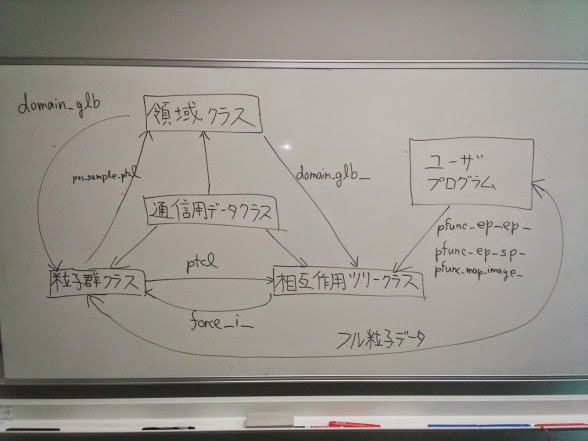
\includegraphics[width=10cm,bb=0 0 600 500]{fig/brief_interface.jpg}
    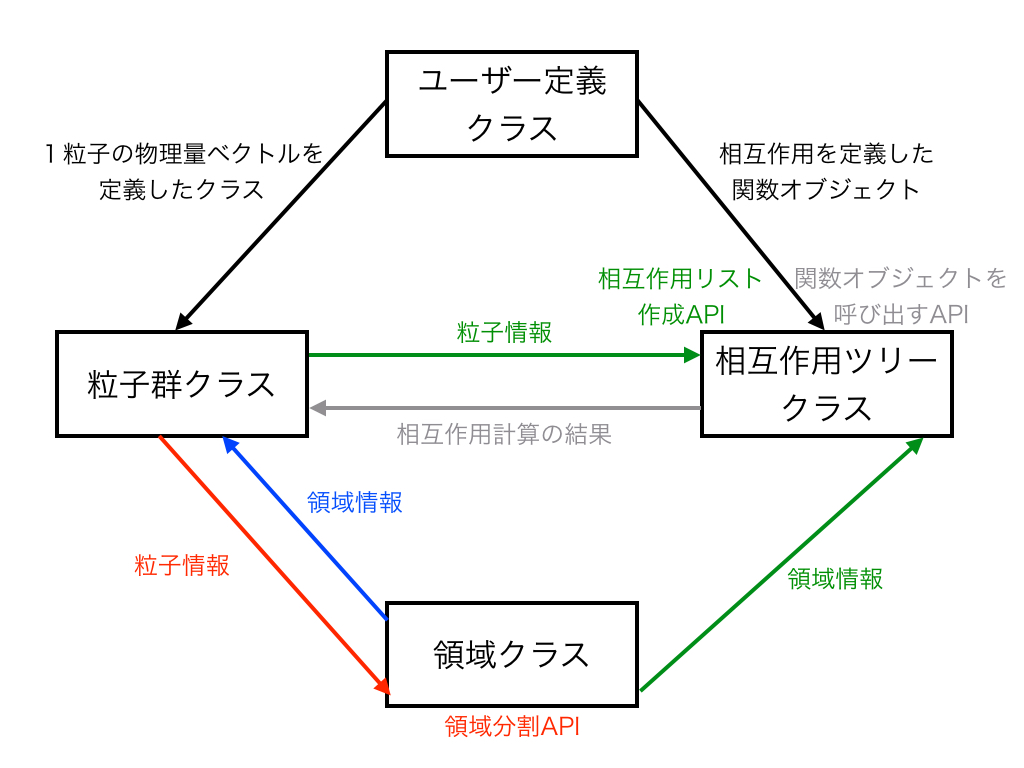
\includegraphics[width=10cm,bb=0 0 700 700]{fig/illustration/illustration.001.jpg}
  \end{center}
  \caption{モジュールインターフェースと情報の流れの模式図。}
  \label{fig:brief_interface}
\end{figure}
